%%%%%%%%%%%%%%%%%%%%%%%%%%%%%%%%%%%%%%%%%%%%%%%%%%%%%%%%%%%%%%%%%%%%%%
% LaTeX Example: Project Report
%
% Source: http://www.howtotex.com
%
% Feel free to distribute this example, but please keep the referral
% to howtotex.com
% Date: March 2011
%
%%%%%%%%%%%%%%%%%%%%%%%%%%%%%%%%%%%%%%%%%%%%%%%%%%%%%%%%%%%%%%%%%%%%%%
% How to use writeLaTeX:
%
% You edit the source code here on the left, and the preview on the
% right shows you the result within a few seconds.
%
% Bookmark this page and share the URL with your co-authors. They can
% edit at the same time!
%
% You can upload figures, bibliographies, custom classes and
% styles using the files menu.
%
% If you're new to LaTeX, the wikibook is a great place to start:
% http://en.wikibooks.org/wiki/LaTeX
%
%%%%%%%%%%%%%%%%%%%%%%%%%%%%%%%%%%%%%%%%%%%%%%%%%%%%%%%%%%%%%%%%%%%%%%
% Edit the title below to update the display in My Documents
%\title{Project Report}
%
%%% Preamble
\documentclass[paper=a4, fontsize=12pt,DIV=14]{scrartcl}    % scrartcl = article-typed dcmt using pckg Koma-script
\usepackage[utf8]{inputenc}

\usepackage[english]{babel}							 % English language/hyphenation
\usepackage[protrusion=true,expansion=true]{microtype}
\usepackage[pdftex]{graphicx}	
\linespread{1}
\usepackage{array}
\usepackage{pdfpages}                               % Packages used to include pdf files
\usepackage{rotating}                               % Allow landscape mode for certain pages

%%% Custom sectioning
\usepackage{sectsty}
\allsectionsfont{\fontfamily{cmss}\selectfont}
\sectionfont{\sectionrule{3ex}{1pt}{-1.5ex}{1pt}}
\subsectionfont{\hspace*{2.5em}}
\paragraphfont{\hspace*{0.5em}}
\subsubsectionfont{\hspace*{5em}}

%Adding snippets of code in a nice way
\usepackage{listings}
\usepackage{color}

\definecolor{dkgreen}{rgb}{0,0.6,0}
\definecolor{gray}{rgb}{0.5,0.5,0.5}
\definecolor{mauve}{rgb}{0.58,0,0.82}

\lstset{frame=tb,
  language=Java,
  aboveskip=3mm,
  belowskip=3mm,
  showstringspaces=false,
  columns=flexible,
  basicstyle={\small\ttfamily},
  numbers=none,
  numberstyle=\tiny\color{gray},
  keywordstyle=\color{blue},
  commentstyle=\color{dkgreen},
  stringstyle=\color{mauve},
  breaklines=true,
  breakatwhitespace=true,
  tabsize=3
}

%%% Custom headers/footers (fancyhdr package)
\usepackage{fancyhdr}
\pagestyle{fancyplain}
\fancyhead[L]{R. Peree, G. Cartier}	% Left page header
\fancyhead[R]{
\includegraphics[scale=0.2]{img/logo.png}
\includegraphics[scale=0.2]{img/via_logo.png}}           % Right page header
\fancyfoot[L]{Autumn 2017}								        % Empty0
\fancyfoot[C]{}									            	% Empty
\fancyfoot[R]{\thepage}							            	% Page numbering
\renewcommand{\headrulewidth}{0pt}		                        % Remove header underlines
\renewcommand{\footrulewidth}{0pt}		                    	% Remove footer underlines
\setlength{\headheight}{20.4pt}
\setcounter{page}{-1}                                           % Starts the page numbering at -1


%%% Begin document
\begin{document}

	%\setlength{\parindent}{0cm}
%\setlength{\parskip}{1ex plus 0.5ex minus 0.2ex}
%\newcommand{\hsp}{\hspace{20pt}}
\newcommand{\HRule}{\rule{\linewidth}{0.5mm}}

\begin{titlepage}
  \begin{sffamily}
  \begin{center}

    
    % Upper part of the page. The '~' is needed because \\
    % only works if a paragraph has started.
    
\includegraphics[scale=0.7]{img/via_logo.png}~\\[1.5cm]

    \textsc{\Large Project Report }\\[1cm]

    % Title
    \HRule \\[0.4cm]
    { \huge \bfseries Surfing-couch\\[0.4cm] }

    \HRule \\[3cm]
    
\includegraphics[scale=0.75]{img/logo.png}\\[1.3cm]

    % Author and supervisor
    \begin{minipage}{0.35\textwidth}
      \begin{flushleft} \large
        Rosalie Peree \textsc{(258377)}\\
      \end{flushleft}
    \end{minipage}
    \begin{minipage}{0.35\textwidth}
      \begin{flushright} \large
        Grégoire Cartier \textsc{(258378)}\\
        %\emph{Chef d'équipe : } M. Chef \textsc{D’Équipe}
      \end{flushright}
    \end{minipage}\\[1.5cm]
    
    \Large\emph{Supervisor \& Academic advisor:} Kasper \& Jakob\textsc{}\\[1cm]


    \vfill

    % Bottom of the page
    {\large 2017 (Autumn semester)}
  \end{center}
  \end{sffamily}
\end{titlepage} %% Titlepage set in titlepage.tex
    \tableofcontents
    \thispagestyle{empty}           %used to remove the page number

    \newpage
        \section*{Abstract} %Title without numbering
        \addcontentsline{toc}{section}{Abstract} %Adding that title without numbering to the toc
        % COMPLETE SECTION TO DO
        % PROOF READ TO DO


    \newpage
        \section{Introduction}
        % COMPLETE SECTION TO DO
        % PROOF READ TO DO
        	\subsection{Background Description}
        	\subsection{Problem Description}
        	\subsection{Limitations and Delimitations}


    \newpage
        \section{Methods}
        % COMPLETE SECTION DONE
        % PROOF READ TO DO
	        \paragraph{}The following table presents our choice of model and methods for the problems that we listed in our project description (see Appendix \#1):
	        \paragraph{}

	        \begin{tabular}{|p{5cm}|p{5cm}|p{5.1cm}|}
	            \hline
                \textbf{What} \newline \textit{Problem} & \textbf{Why} \newline \textit{Why study this problem} & \textbf{Which} \newline \textit{Which models/theories did you use to solve the problem?}\\
                \hline
                \hline
                How can we develop a social application which is fun to use and rewards the user for helping travellers in their area? 
                & How to make the application interesting for our potential users?
                & We have to pay attention to all the following problems to be able to develop an application that will address all of them as good as possible.\\
                \hline
                What is important for travellers?
                & As our application is mainly targeted to travellers, it is interesting to know what is important for them, so that we cant try to implement those things in the final application.
                & We conducted a survey via Google Forms to gather people's opinion on that subject.\\
                \hline
                What is important for hosts?
                & As we want hosts to offer services to travellers, we have to meet with what they want to encourage them to do so.
                & We conducted a survey via Google Forms to gather potential user's opinion on that subject.\\
                \hline
                How can we allow users to create and find trips in their area and offer a service to travellers?
                & This problem is the main problem for a couch-surfing-like application. We have to localize the user to be able to provide a service for them in a specific area.
                & We have to set up a way for the users to enter their city/location and look for hosts in cities they want to visit.\\
                \hline
                How can we make the service secure for users?
                & Users don't want their personal data to be forwarded to strangers.
                & No personal data is displayed on the application for users to see. We implemented an internal messaging system so people can communicate directly on the application.\\
                \hline
                Can we add reviews and comments about travellers and hosts?
                & If you have to host someone or sleep/shower at a stranger's place, safety is very important. Users need a way to see if someone behaved correctly or not before their stay.
                & We implemented a system of user reviews - with grades - so people can report how they experience was with that specific user - hosts and travellers.\\
                \hline
            \end{tabular}

            \begin{tabular}{|p{5cm}|p{5cm}|p{5cm}|}
	            \hline
                \textbf{What} \newline Problem & \textbf{Why} \newline Why study this problem & \textbf{Which} \newline Which models/theories did you use to solve the problem?\\
                \hline
                \hline
                How can we define the point-value of the provided services?
                & As the system is based on a reward, all services must have a fixed value.
                & We defined a value for each service - sleep, shower and laundry. The points are given to the host once the booking is completed.\\
                \hline
                How can we exchange the points for gifts?
                & The system is based on rewarding hosts with gifts for providing a service.
                & We set up an online shop where users can exchange their points for goods.\\
                \hline
                How will the user interface be implemented?
                & The user interface has to be easy to get and use.
                & The interface will be an Android application.\\
                \hline
                What kind of tool will be used for this implementation?
                & The tools used to develop can make the process of developing the application more or less easy.
                & We decided to develop the application using Android Studio, as it is the platform we are both most familiar with.\\
                \hline
                How will the interface be user-friendly?
                & The interface has to be easy to use and understand for any user.
                & The interface is simple, with buttons and labels that are easy to understand. \\
                \hline
                How is the social interaction going to take place?
                &The point of the assignment is to enable a social interaction.
                & In our application, the social interaction will take place in the form of direct messaging between two users, a common chat for all the users and the possibility of reviewing experience with other users.\\
                \hline
                What kind of database will be implemented?
                & We need a database that is free and easy to integrate in Android.
                & The chosen database is Firebase for our project.\\
                \hline
            \end{tabular}


    \newpage
        \section{Requirements}
        % COMPLETE SECTION DONE
        % PROOF READ TO DO
        	\paragraph{}The users of the application will be any person interested in traveling on a budget or having a different traveling experience, as well of any person that will be willing to host or provide a service -for now, shower and laundry - to a traveller visiting their city. They could be from everywhere in the world and have about any age, as long as they have access to a mobile phone running Android and a working Internet connection. They should not have an extensive knowledge of computer science to be able to use the application.
        	\subsection{List of Requirements}
        		\paragraph{}Before starting any implementation, we conducted a survey to gather some data about potential users. Here are some of the results that could be interesting:
        		\begin{itemize}
        			\item \textbf{More than 70\%} of the people that replied are using an Android phone. Developing a native Android application seems to be a good strategic choice.
        			\item Again, \textbf{more than 70\%} of the people would be interested to collect rewards by hosting someone. For \textbf{3\/4 th} of those people, it would also depend of the rewards.
        			\item For \textbf{more than 50\% }of the travellers, safety is the most important.
        			\item For \textbf{20\% }of our potential hosts, getting a reward would encourage them to host people in their home.
        			\item For more statistics, refers to graphics in Annex B.
        		\end{itemize}
    \newpage
        		\subsubsection{Functional Requirements}
        			\paragraph{Use cases:}
        			\paragraph{}

		                \begin{figure}[!htbp]
		                    \center
		                    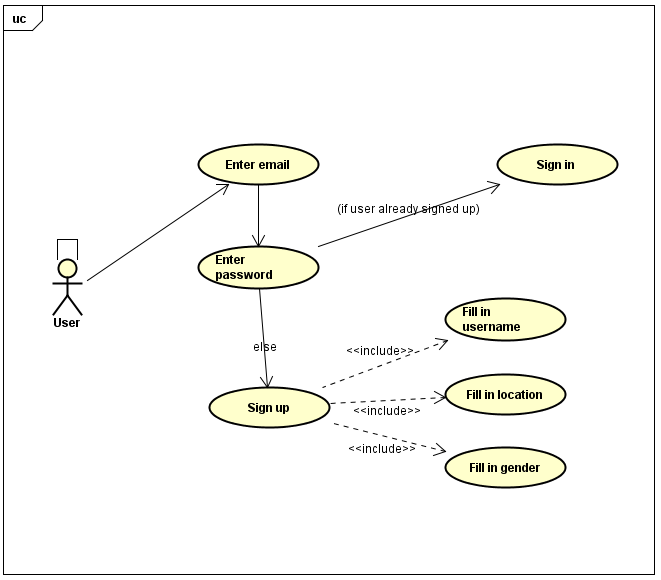
\includegraphics[scale=0.75]{img/enter_application.png}
		                    \caption{Use Case 1: how to access to application}
		                \end{figure}

		                \begin{figure}[!htbp]
		                    \center
		                    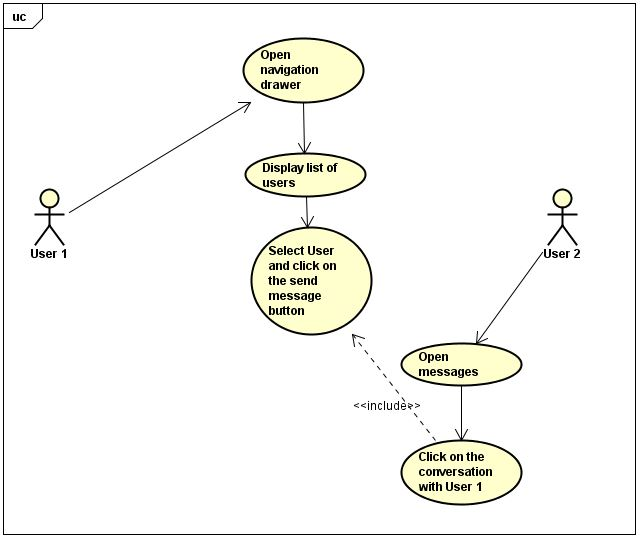
\includegraphics[scale=0.7]{img/send_message.png}
		                    \caption{Use Case 2: how users can communicate together by messages}
		                \end{figure}

		                \begin{figure}[!htbp]
		                    \center
		                    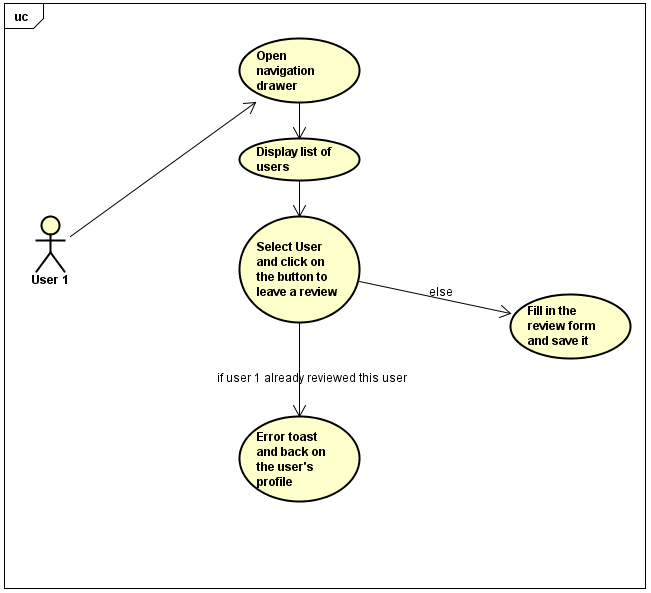
\includegraphics[scale=0.7]{img/leave_review.png}
		                    \caption{Use Case 3: how a user can leave a review to another user}
		                \end{figure}

		                \begin{figure}[!htbp]
		                    \center
		                    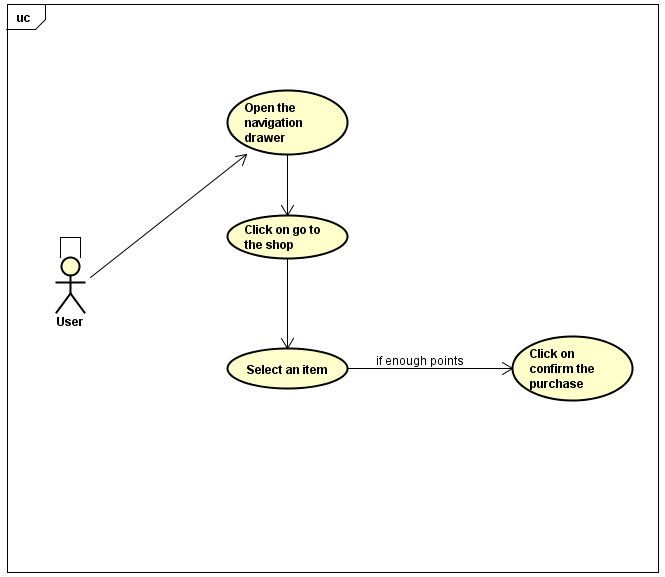
\includegraphics[scale=0.75]{img/shop.png}
		                    \caption{Use Case 4: how a user can cash his points for a reward}
		                \end{figure}
\newpage
		                \paragraph{Activity Diagrams:}
        				\paragraph{}

		                \begin{figure}[!htbp]
		                    \center
		                    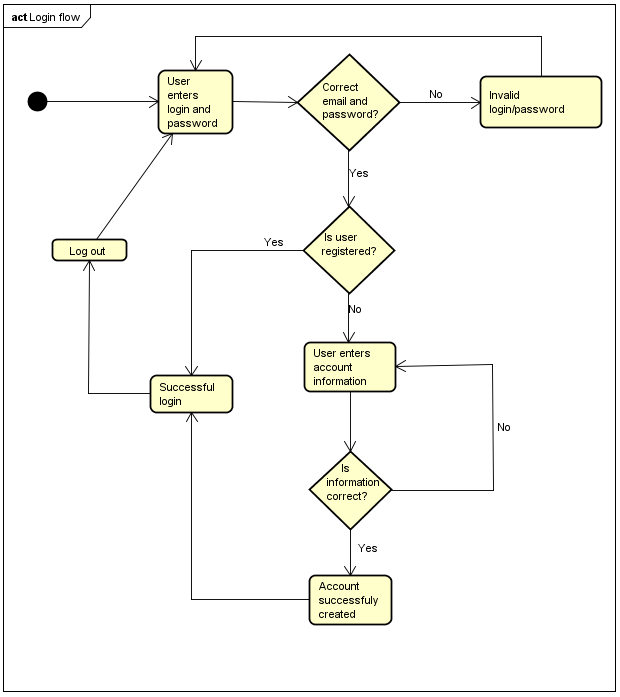
\includegraphics[scale=1]{img/act_login.png}
		                    \caption{Activity Diagram 1: sign in on the application}
		                \end{figure}
		                \newpage

		                \begin{figure}[!htbp]
		                    \center
		                    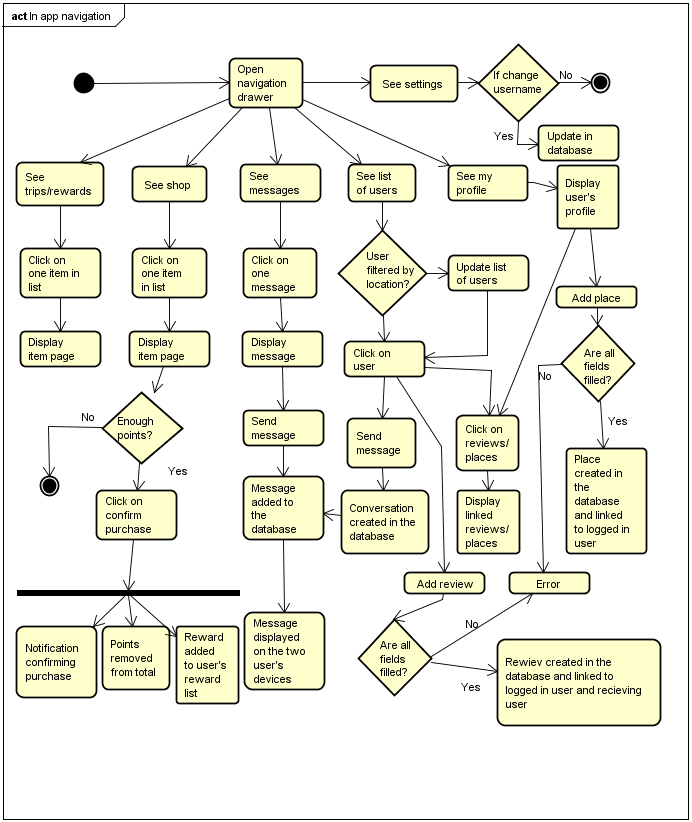
\includegraphics[scale=1]{img/act_navigation.png}
		                    \caption{Activity Diagram 2: navigation from the navigation drawer}
		                \end{figure}

		                \paragraph{}The second activity diagram groups some activities together. The activities that are merged together on the diagram are distinct activities, but have the same behavior and thus can be grouped together. This is done to avoid this diagram to become too complicated to read.

        		\subsubsection{Non-Functional Requirements}
        			\paragraph{Security}
        			\begin{itemize}
        				\item Password requirements (set up by Firebase)
        				\item Password security (hashed)
        				\item Password not saved unencrypted
        				\item If password lost, email to make a new one (handled by Firebase)
        			\end{itemize}
        			\paragraph{Usability}
        			\begin{itemize}
        				\item User friendly
        				\item Possible translation of the application due to avoiding hard-coded strings
        			\end{itemize}

    \newpage
        \section{Analysis}
        % COMPLETE SECTION DONE
        % PROOF READ TO DO
            \begin{figure}[!htbp]
                \center
                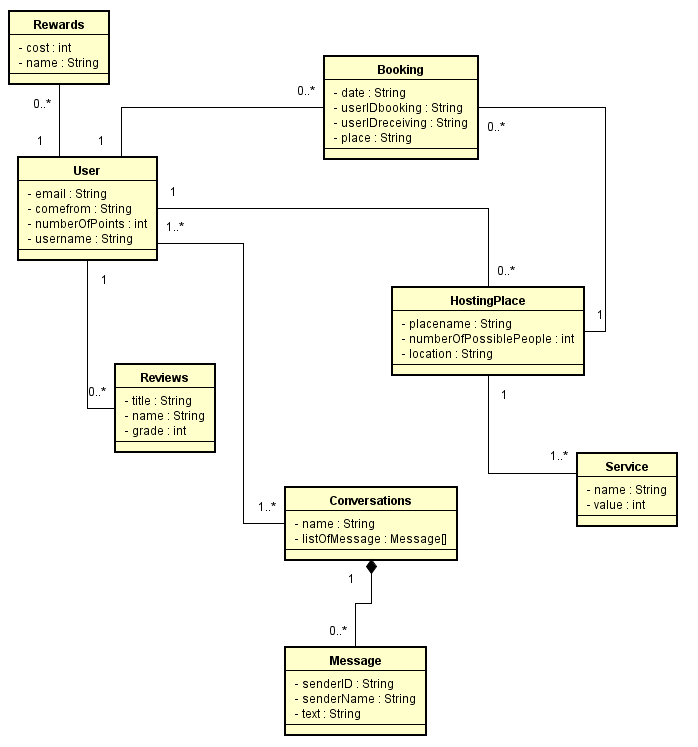
\includegraphics[scale=0.9]{img/domain_model.png}
                \caption{Domain model}
            \end{figure}
            \paragraph{}The domain model represents the basic structure that we want our application to have and the requirements that we want it to be able to complete.

    \newpage
        \section{Design}
        % COMPLETE SECTION TO DO
        % PROOF READ TO DO
        	\subsection{Architecture}
				\paragraph{}We used the Adapter in Android which is close to a Pattern Adapter.

				\begin{figure}[!htbp]
					\center
		            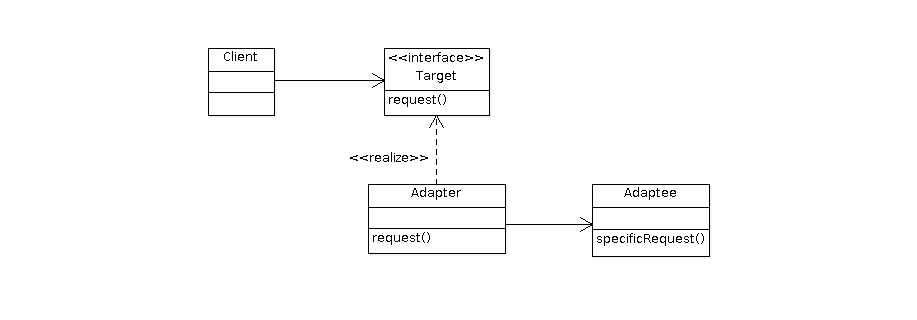
\includegraphics[scale=0.5]{img/adapterpattern.png}
		            \caption{Adapter Pattern Template (\textit{softwarepassion.com})}
				\end{figure}

				\paragraph{}We used those Adapters to populate the listViews with ArrayList and make clickable. Those Adapters are customizable, and help to display the content of the Objects that are kept in the database 

				\paragraph{}We also wanted to use a MVC (Model View Controller), which is a MVP (Model View Presenter) but the scope of the project was too short to implement it correctly, and we didn't studied it during the Android course.

        	\newpage
        	\subsection{Technologies}
        		
				\paragraph{}\textbf{Surfing Couch} uses different technologies :\\
				\paragraph{}To do deal with all of the data manipulated by the users, the applications uses \textbf{Firebase} as database : \\
				\begin{itemize}
					\item Pros :
						\begin{itemize}
						\item 	Firebase provides an easy implementation on an Android application, there is not that much of a setup to do, the read and write functions are really easy to implement
						\item 	Firebase use JSON which permits an implementation of data in a fairly effortless way. That create a database that is flexible, well-structured and easy to read to some extent.
						\item 	Firebase gives useful tools, including a user authentication that deals with the security of database thanks to its data hashing. Firebase is also loaded with email confirmation, data analytics, and stability tools, which helps to make the user experience better.
						\item 	Made by Google
						\end{itemize}

					\item Cons :
						\begin{itemize}
						\item	When the data structure starts to be a bit complex, it becomes quite hard to navigate through all of the data. Especially if you have a lot of data.
						\item	The querying and indexing is very limited due to the use of the JSON. It makes the search of data is very redundant.
						\item	Firebase is a bit high level, so you don’t feel you have that much of control over it
						\item	Made by Google
						\end{itemize}
				\end{itemize}

				\paragraph{}One of the alternative to Firebase could be to use a more “classical” database management system like \textbf{SQLite} :
				\begin{itemize}
					\item Pros :
						\begin{itemize}
							\item	Classical way to store data, you can do SQL queries on it to retrieve data with more efficiency. Include also a good indexing of the data.
							\item	Is better than Firebase at storing huge load of data.
						\end{itemize}
					\item Cons :
						\begin{itemize}
							\item	You don’t have the tools proposed by Firebase, so you can really analyze your data usage and you must make all of the part of the security by yourself
							\item	Harder to use and implement than Firebase.
						\end{itemize}
				\end{itemize}

				\paragraph{}The application must be developed natively on Android, so \textbf{Android Studio} was a default choice to develop the application. But it's interesting to point out that there is alternatives to Android Studio such as \textbf{Xamarin} or \textbf{Cordova}.

			\subsection{Design Patterns, Class Diagram, Sequence Diagrams}

				\paragraph{}Like said earlier, we are not using a specific design pattern.

					\begin{figure}[!htbp]
						\center
	                    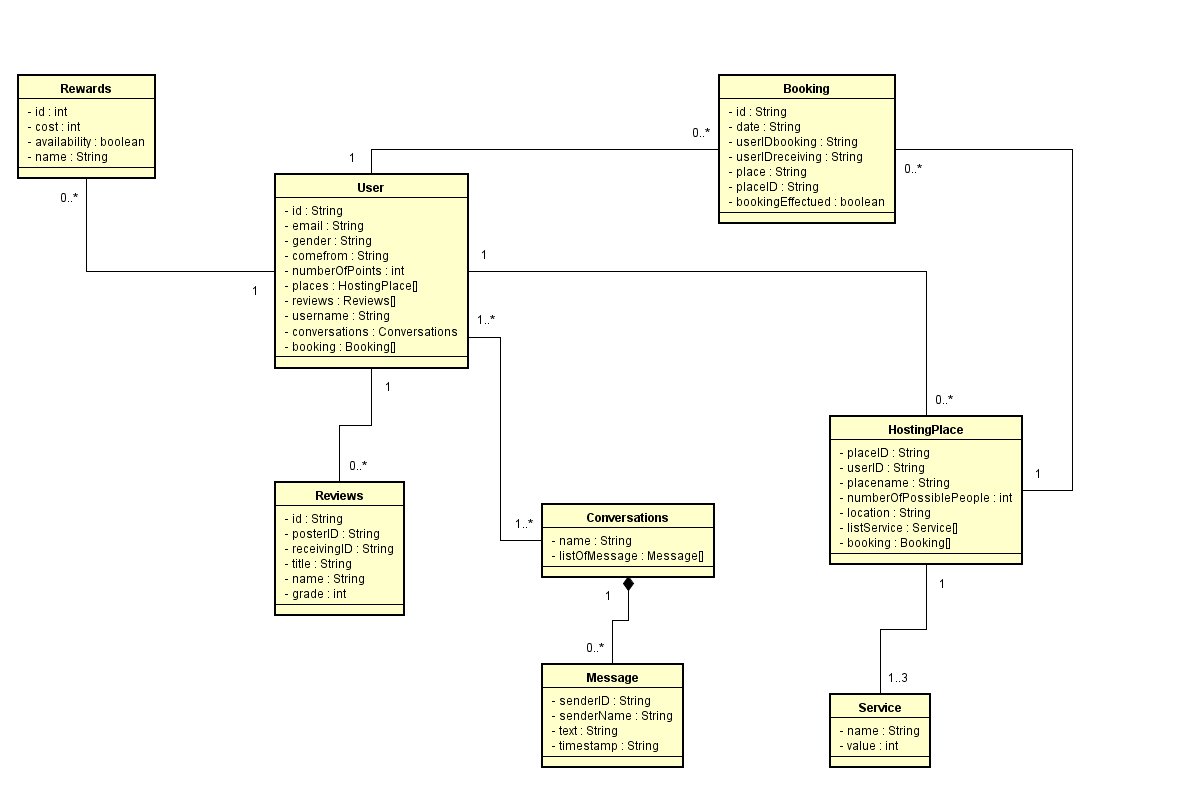
\includegraphics[scale=0.6]{img/class_diagram.png}
	                    \caption{Class Diagram of the database } 
					\end{figure}

				\paragraph{}The database\footnote{We made a class diagram for the database because the data is kept in a JSON} is pretty straightforward, everything is based around the User. However, we must highlight some details. By default, when a user is created, the bookings are null, so not present in the database JSON. The list is created with the first booking he makes.
				\paragraph{}Also, a default chat is assigned to each user which is the “General Chat” so can talk all together. The other List are defined as “undefined” and taken as HashMaps inside of the application.
				
						\begin{sidewaysfigure}[!htbp]
							\center
		                    \includegraphics[scale=0.55]{img/activity.png}
		                    \caption{Class Diagram of the application Activities } 
						\end{sidewaysfigure}
				\paragraph{}All of the activities apart from the MainActivity and the Adapter are extending the NavigationDrawerActivity which is itself extending AppCompatActivity.
				\paragraph{}A user can add review only once per User, and some Display activities are accessible according if you are on your profile or someone else profile
				\paragraph{}Each Activities have an OnCreate() function and other (OnStart(), OnStop()), since those methods are part of the life cycle there aren’t displayed.
				\paragraph{}Each Adapter have overridable methods, that are also not displayed on the diagram


    \newpage
        \section{Implementation}
        % COMPLETE SECTION TO DO
        % PROOF READ TO DO
\begin{lstlisting}
        DatabaseReference ref = reference.child("User/"+FirebaseAuth.getInstance().getCurrentUser().getUid());

    ref.addListenerForSingleValueEvent(new ValueEventListener() {
        @Override
        public void onDataChange(DataSnapshot dataSnapshot) {

            user = dataSnapshot.getValue(User.class);
            if (user.getConversations() == null) {
                Toast.makeText(getApplicationContext(), R.string.message_empty, Toast.LENGTH_SHORT).show();

            } else {
                        allChats.clear();
                for (String value : user.getConversations().values()) {
                    allChats.add(value); //This also add in adapter at the same time
                    listOfChats.setAdapter(adapter);
                }

            }
        }

        @Override
        public void onCancelled(DatabaseError databaseError) {
            Toast.makeText(getApplicationContext(), R.string.message_error, Toast.LENGTH_SHORT).show();
        }
    });
	\end{lstlisting}
	\paragraph{}We can access to the message in two different ways. The first way is to pass through the MessageActivity, which display the list of the conversation that the connected user possesses. By default, the user has the ``''General Chat``''. He just has to click on the name of the chat to open it thanks to the \textbf{MessageAdapter}.
\paragraph{} When the User accesses the \textbf{MessageActivity}, we create a reference on the database and the put a \textit{addListenerForSingleValueEvent} to fetch the data from the Database. We use the \textit{snapshot} to retrieve the \textbf{User} data and then we store the data inside of an array that we put inside of an adapter that is used to display the data in the ListView
\begin{lstlisting}
    listOfChats.setOnItemClickListener(new AdapterView.OnItemClickListener() {
        @Override
        public void onItemClick(AdapterView<?> adapterView, View view, int i, long l) {
            Intent intent = new Intent();
            intent.setClass(getApplicationContext(),ChatActivity.class);
            intent.putExtra("position", i);

            intent.putExtra("chatName", listOfChats.getItemAtPosition(i).toString());
            startActivity(intent);
        }
    });

        	\end{lstlisting}

        	\paragraph{}When the user clicks on a chat name, we get the position of the click and the name of the chat selected, that we send into an intent to open the chat. The intent will be used to open the correct chat.
			\paragraph{}If no chat exists between some users, a user can go the profile of someone and click on send message to create a conversation and use CheckConversationActivity.

\begin{lstlisting}
if(currentUser.getConversations() != null || displayedUser.getConversations() != null) {
    loop:
    {
        for (String conv : currentUser.getConversations().values()) {
            for (String conv2 : displayedUser.getConversations().values()) {
                if (Objects.equals(conv, conv2) && !Objects.equals(conv, "General Chat")) {

                    intent.putExtra("chatName", conv2);
                    startActivity(intent);
                    break loop;
                }
            }
        }

        ref.child(currentUser.getUsername() + " - " + displayedUser.getUsername()).setValue(currentUser.getUsername() + " - " + displayedUser.getUsername());
        ref2.child(currentUser.getUsername() + " - " + displayedUser.getUsername()).setValue(currentUser.getUsername() + " - " + displayedUser.getUsername());
        intent.putExtra("chatName", currentUser.getUsername() + " - " + displayedUser.getUsername());
        startActivity(intent);
    }

}else {
    ref.child(currentUser.getUsername() + " - " + displayedUser.getUsername()).setValue(currentUser.getUsername() + " - " + displayedUser.getUsername());
    ref2.child(currentUser.getUsername() + " - " + displayedUser.getUsername()).setValue(currentUser.getUsername() + " - " + displayedUser.getUsername());
    intent.putExtra("chatName", currentUser.getUsername() + " - " + displayedUser.getUsername() );
    startActivity(intent);
}


        	\end{lstlisting}

        \paragraph{}In this activity, we check a conversation exists between two users. If the conversation doesn’t exist between the users. If doesn’t we write into the database this new conversation and then send the user on the ChatActivity


        	\begin{lstlisting}
        		sendButton.setOnClickListener(new View.OnClickListener() {
    @Override
    public void onClick(View view) {
        if (sendText.getText().toString().trim().length() == 0) {
            Toast.makeText(ChatActivity.this, R.string.chat_empty_text, Toast.LENGTH_SHORT).show();
        } else {
            SimpleDateFormat sdf = new SimpleDateFormat("dd/MM/yyyy - HH:mm", Locale.FRANCE);
            String currentDateAndTime = sdf.format(new Date());
            FirebaseDatabase.getInstance().getReference().child("Conversation/" + chatName + "/listOfMessages").push().setValue(new Message
                    (
                    FirebaseAuth.getInstance().getCurrentUser().getUid()
                    , lul.getUsername()
                    , sendText.getText().toString()
                    , currentDateAndTime
                    )
            );
            sendText.setText("");
        }
    }
});

        	\end{lstlisting}

        	\paragraph{} This is an example of how the writing a message is made. 
			\paragraph{}At first, we are checking if the input field of the user is empty or not. We have to trim it in case of the User just put a blank space. 
			\paragraph{}If the input field is not empty, we can fetch the date and the time at the moment the send button was pressed, and we write all of the relevant data into the database and then we empty the input field.
			\paragraph{}To write in the database, we have to get a reference on the database and then look for where we want to write the data which here is: 'Conversation\/>chat\_name>\/listOfMessages'
			\paragraph{}The push value will add a new instance of the object \textbf{Message} that contains a UserID, a username, the user text and a timestamp.

			\begin{lstlisting}
public class Message {
    protected String senderID;
    private String senderName;
    private String text;
    private String timestamp;
    }

        	\end{lstlisting}





    \newpage
        \section{Test}
        % COMPLETE SECTION DONE
        % PROOF READ TO DO
        	\subsection{Test Specifications}
        		\paragraph{}Because of the specification of our application and the fact that we did not go through testing during class, we decided to go with black box testing and a user testing, because our application is supposed to have a focus on an intuitive user interface.
        	\subsection{Black Box Testing}
            \begin{tabular}{|p{4.3cm}|p{4.3cm}|p{4.3cm}|p{2cm}|}
	            \hline
                \textbf{Test}& \textbf{Expected Result} & \textbf{Actual Result} & \textbf{Status} \\
                \hline
                \hline
                Login 
                & Success
                & Success
                & Passed \\
                \hline
                Login with wrong password
                & Password not matching the password in the database
                & Password not matching error
                & Passed\\
                \hline
                Login with password too short
                & Password less than 6 characters: error
                & Password too short error
                & Passed\\
                \hline
                Email address not correct
                & Email address not correctly formatted
                & Email address formatted badly error
                & Passed\\
                \hline
                Email address not already registered
                & Can't sign in with given email address
                & No user corresponding to this email address
                & Passed\\
                \hline
                Create account not allowed if address is already registered
                & Can't create account if already have an account
                & Email address already in use with another account
                & Passed\\
                \hline
                Create an account without filling all the fields
                & Not allowed to create an account
                & Error because all the fields are not filled
                & Passed\\
                \hline
                Go back to sign in activity after signing in by using the back button and not the logout button
                & Application closing
                & Application closing
                & Passed\\
                \hline
                Confirm email address
                & The user has to confirm their email address before having access to the application
                & It is not possible for the user to access the application without having confirmed their email address
                & Passed\\
                \hline
                Display User's profile
                & Display profile of user with data saved in the database
                & Display profile of user with data saved in the database
                & Passed\\
                \hline
                Have only button "add place" on logged user's profile
                & Button "write message" not displayed on logged user's profile
                & Button "write message" not displayed on logged user's profile
                & Passed\\
                \hline
            \end{tabular}

			\begin{tabular}{|p{4.3cm}|p{4.3cm}|p{4.3cm}|p{2cm}|}
	            \hline
                \textbf{Test}& \textbf{Expected Result} & \textbf{Actual Result} & \textbf{Status} \\
                \hline
                \hline
                Add a place without filling all the fields should not be allowed
                & Not saving into database and output an error if the user attempts to create a place without all the fields 
                & Error outputs as a toast and the data is not saved until all the fields are completed
                & Passed\\
                \hline
                Display all of my trips
                & Display list of my bookings, if list is empty, display nothing. Avoid crashing the application
                & The application is not crashing even if there is no booking
                & Passed\\
                \hline
                Display all of my rewards
                & Display list of my rewards, if list is empty, display nothing. Avoid crashing the application
                & The application is not crashing even if there is no rewards
                & Passed\\
                \hline
                Display the items in the shop with Grey background and not clickable if item is not available
                & The non-available items in the shop should not be activated
                & The non-available items in the shop are with Grey background and can't be clicked
                & Passed\\
                \hline
                Allowing buy of items in the shop only if the amount of points the user has is enough
                & If the user does not have enough points, the button for the buy is not activated
                & Button not activated if the user does not have enough points
                & Passed\\
                \hline
                Allowing the purchase if item available and user has enough points
                & The item can be purchased
                & The item ca be purchased
                & Passed\\
                \hline
                Removing the points from the total amount of points the user has when a purchase is made
                & The points are deduced from the amount of points the user has
                & The point are correctly deduced
                & Passed\\
                \hline
                Notifying the user that the purchase has been made
                & Give an alert to the user to tell them that the purchase was successful
                & Send a notification once a purchase has successfully been made to inform the user
                & Passed\\
                \hline
                Check the user's messages
                & The logged in user should be able to get a list of the messages he got
                & The list of messages is accessible to the user via the navigation drawer
                & Passed\\
                \hline
                Send a message to another user via an existing conversation
                & The conversation should update on both phones and display correctly
                & The conversation displays on both phones and refreshes once a message is sent
                & Passed\\
                \hline
                List all the users that are using the application
                & Being able to see all the users in a list
                & The users are all displayed in a list
                & Passed\\
                \hline
            \end{tabular}


			\begin{tabular}{|p{4.3cm}|p{4.3cm}|p{4.3cm}|p{2cm}|}
	            \hline
                \textbf{Test}& \textbf{Expected Result} & \textbf{Actual Result} & \textbf{Status} \\
                \hline
                \hline
                Filter users in a specific area
                & We have to be able to filter the user list to keep only users in one area - to be able to look for a host for your next trip
                & The filter allows you to filter using a Google Map location
                & Passed\\
                \hline
                Send a message to another user
                & The users have to be able to send a message to another user by navigating to the user's profile
                & The button "send a message" is displayed and allows to send a message to the user - if a conversation exists already, this one is opened.
                & Passed\\
                \hline
                Leave a review to an user
                & Being able to review another user
                & It is possible to review an user using the button on their profile
                & Passed\\
                \hline
                Review another user multiple times
                & It should be possible to review someone just once to avoid fake reviews
                & If a review has already been added for that user, the system does not allow the user to send a new review
                & Passed\\
                \hline
                Send an empty review 
                & It should not be possible to send a review without filling out all the fields
                & All the fields have to be filled for the review to be sent
                & Passed\\
                \hline
                Display the user's data in the setting activity
                & The settings page has to display the correct data
                & The settings page displays the data that is in the database
                & Passed\\
                \hline
                Change the settings
                & The user has to be able to change their username in the settings
                & When the user changes their username in the settings, it changes it in the database and refresh the data displayed on the settings page
                & Passed\\
                \hline
                Log out of the application
                & The user has to be able to log out successful from the application and be redirected to the login screen
                & The user is logged out and redirected to the login screen
                & Passed\\
                \hline
                Pressing the back button after logging in
                & The user should not be able to go back to the inside of the application without logging in again
                & If the user tries to go back after logging out, the application stops
                & Passed\\
                \hline
            \end{tabular}

            \subsection{User test}
            %insert what Leo said about the application 



    \newpage
        \section{Results \& Discussion}
        % COMPLETE SECTION TO DO
        % PROOF READ TO DO



    \newpage
        \section{Conclusion}
        % COMPLETE SECTION TO DO
        % PROOF READ TO DO


        %\newpage
\setlength{\parindent}{0cm}
\section{Sources, references and literature}
    \subsection{Definitely:}
        \begin{itemize}
%            % Marketing Bibliography
%            \item[] McDonald, Malcolm H.B. and Wilson, Hugh. 2016. \textit{Marketing plans: how to prepare them, how to use them.} Chichester: Wiley.
%            \item[] Belz, Frank-Martin and Peattie, Ken. 2009. \textit{Sustainability marketing: a global perspective.} Chichester: Wiley.
%            % ICT bibliography
%            \item[] Ford, J. (2009). \textit{Ajax programming for the absolute beginner.} 1st ed. Boston, MA: Course Technology Cengage Learning.
 %           \item[] Hazem, S. (2014). \textit{JavaScript Mobile Application Development.} 1st ed. Birmingham B3 2PB, UK.: Packt Publishing Ltd.
 %           \item[] Kumar Patel, S. (2014). \textit{Developing responsive web applications with AJAX and jQuery.} 1st ed. Birmingham, U.K: Packt Pub.
%            \item[] Montoro, A. (2011). \textit{IPhone JavaScript cookbook.} 1st ed. Birmingham, U.K.: Packt Pub.
 %           \item[] Shotts, K. (2014). \textit{PhoneGap 3.x Mobile Application Development Hotshot.} 1st ed. Birmingham: Packt Publishing.
%            \item[] Vohra, D. (2015). \textit{JavaServer Faces 2.0.} 1st ed.
%            \item[] Wagner, R. (2009). \textit{JavaScript \& Ajax for dummies.} 1st ed. New York: Wiley.
         \end{itemize}
    \subsection{Possibly:}
        \begin{itemize}
            % Marketing Bibliography
%            \item[] Comm, Joel and Taylor, David. 2015. \textit{Twitter power 3.0: how to dominate your market one tweet at a time.} Hoboken: Wiley.
%            \item[] Ruey-Jer Bryan Jean, Jyh-Shen Chiou and Shaoming Zou. 2013. \textit{International marketing in rapidly changing environments.} Bingley: Emerald.
%            \item[] Viardot, Eric. 2004. \textit{Successful marketing strategy for high-tech firms.} Boston: Artech House.
%            \item[] Shaoming Zou, Hui Xu and Linda Hui Shi. 2015. \textit{Entrepreneurship in international marketing.} Bingley: Emerald.
%            \item[] Stöttinger, Barbara, Schlegelmilch, Bodo B. and Zou, Shaoming. 2015. \textit{International marketing in the fast changing world.} Bingley: Emerald.
%            \item[] Chang, C.M. 2014. \textit{Business fundamentals for engineering managers.} New York: Momentum Press.
        \end{itemize}
\newpage                             % Adding the sources page

%%% End document
\end{document} 